\documentclass[a4paper]{article}

\usepackage[utf8]{inputenc}
\usepackage[T1]{fontenc}
\usepackage{textcomp}
\usepackage{listings}
\usepackage{lmodern}
\usepackage{amsfonts}
\usepackage{titling}
\usepackage{lipsum}
\usepackage[left=1in, right=1in, bottom=1in, top=1in]{geometry}
\usepackage{amsthm}
\usepackage{tcolorbox}
\usepackage{hyperref}
\usepackage{xcolor}
\usepackage{graphicx}
\usepackage{makeidx}
\usepackage{tikz}
\usepackage{cases}
\usepackage{apacite}
\usepackage{tkz-berge}
\usepackage{url}
\usepackage{tgtermes}
\usepackage{sectsty}
\usepackage{subcaption}
\usepackage{setspace}
\usepackage{float}
\usepackage{amsmath, amssymb}


% figure support
\usepackage{import}
\usepackage{xifthen}
\pdfminorversion=7
\usepackage{pdfpages}
\usepackage{transparent}
\usepackage{color}
\newcommand{\incfig}[2][1]{%
    \def\svgwidth{#1\columnwidth}
    \import{./figures/}{#2.pdf_tex}
}
\newcommand\mapsfrom{\mathrel{\reflectbox{\ensuremath{\mapsto}}}}
%mathstyling
\theoremstyle{plain}
\newtheorem{thm}{Theorem}[section]
\newtheorem{lem}[thm]{Lemma}
\newtheorem{prop}[thm]{Proposition}
\newtheorem*{cor}{Corollary}
\newcommand*{\MyDef}{\mathrm{def}}
\newcommand*{\eqdef}{\ensuremath{\mathop{\overset{\MyDef}{=}}}}
\theoremstyle{definition}
\newtheorem{defn}{Definition}[section]
\newtheorem{conj}{Conjecture}[section]
\newtheorem{exmp}{Example}[section]
\newtheorem{axiom}{Axiom}
\theoremstyle{remark}
\newtheorem*{rem}{Remark}
\newtheorem*{note}{Note}

\definecolor{darkgreen}{rgb}{0.0, 0.5, 0.0}

\pdfsuppresswarningpagegroup=1
\lstset{
tabsize = 4, %% set tab space width
showstringspaces = false, %% prevent space marking in strings, string is defined as the text that is generally printed directly to the console
numbers = left, %% display line numbers on the left
commentstyle = \color{darkgreen}, %% set comment color
keywordstyle = \color{blue}, %% set keyword color
stringstyle = \color{red}, %% set string color
rulecolor = \color{black}, %% set frame color to avoid being affected by text color
basicstyle = \small \ttfamily , %% set listing font and size
breaklines = true, %% enable line breaking
numberstyle = \tiny,
  frame=none,
  xleftmargin=2pt,
  stepnumber=1,
  belowcaptionskip=\bigskipamount,
  captionpos=b,
  escapeinside={*'}{'*},
  language=haskell,
  tabsize=2,
  emphstyle={\bf},
  showspaces=false,
  columns=flexible,
  showstringspaces=false,
  morecomment=[l]\%,
}
\begin{document}
	\begin{titlepage}
	\begin{center}
	\large
	University of Warwick \\
	Department of Computer Science \\
	\huge
	\vspace{50mm}
	\rule{\linewidth}{0.5pt} \\
	CS260 \\
	\vspace{5mm}
	\Large
	Algorithms	
	\rule{\linewidth}{0.5pt}
	\vspace{5mm}
	\begin{figure}[H]
	\centering
	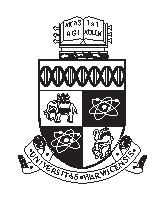
\includegraphics[width=0.4\textwidth]{crest_black.eps}
	\end{figure}
	\vspace{37mm}
	Cem Yilmaz \\
	\today
	\end{center}
	\end{titlepage}	
	\tableofcontents
	\section{Revision}
	\subsection{Past Paper}
	\begin{itemize}
		\item 2019 - questions 1, 5a, 6e, 7, 8
		\item 2020 - questions 1a, 5d-e, 6, 7a-c, 8c-d
		\item 2021 - questions 1
	\end{itemize}
	\subsection{Books}
	Algo design by eva jordan
	chapters 4,5,6,8,7, 4.1
	background using chapters 2,3

	\section{Greedy Algorithms}
	Typically in a greedy algorithm:
	\begin{itemize}
		\item They are efficient to compute
		\item Most 'greedy rules' yield incorrect algorithms. This is why we justify correctness.
	\end{itemize}
	\subsection{Greedy Rules}
		\begin{enumerate}
			\item Earliest start time first (ESTF) 
			\item Shortest first (SF)
			\item Fewest incompatibilities first (FIF)
			\item Earliest finish time first (EFTF)
		\end{enumerate}
	\section{Interval Scheduling}
	The point of the interval scheduling problem is that we attempt to find disjoint intervals. That is, where an interval is a "job", we try to find which jobs are compatible, as you cannot be in two rooms at the same time. The goal is to maximise the number of jobs.
	\begin{lstlisting}[language = Pseudocode , caption={Interval Scheduling} , frame = trBL , firstnumber = last , escapeinside={(*@}{@*)}]
		Initialise the set (*@$I$@*) where (*@$I=[n]\eqdef \{1,2,\ldots,n\}$@*). Let us initialise the answer set (*@$A = \varnothing$@*).
		while (*@$I \neq \varnothing $@*) do: 
			pick (*@$i \in I$@*) using a "greedy" rule 
			add (*@$i$@*) to (*@$A$@*) 
			delete (*@$i$@*) from (*@$I$@*) together with all jobs that are incompatible with job (*@$i$@*).
		return (*@$A$@*).
	\end{lstlisting}

	\begin{itemize}
		\item Input - $n$ open intervals where intervals denoted by $(s(1),f(1)),(s(2),f(2)),\ldots (s(n), f(n))$ where $s(n)<f(n)$ and $f(n)=  s(n+1)$.
		\item Output - $S \subseteq [n] =^\text{def} \{1,2,\ldots,n\}$
	\end{itemize} 
	Q: how to check ine $O(1)$ time of jobs $i,j$ are compatible (disjoint) \\
	$s(i) > f(j)$, $s(j) > f(i)$
	\subsection{Algorithm Correctness}
	\begin{enumerate}
		\item Fact 1 - $A$ is compatible, that is, whenever we add $i$, we remove incompatibilities, therefore $A$ is compatible.
		\item Fact 2 - is a theorem which is found below.
		\item Fact 3 -"$A$ stays ahead of $C$"
	\end{enumerate}
	\begin{thm}
		$A$ is optimal, that is, largest size $A$ that is compatible.
			One way to show that is that the answer $A$ is equal to $O$, the optimal set. However, this idea is not too good since $O$ is not necessarily unique. \\
			However, there is a work around. It is to show that $|A| \ge |C|$ for any compatible set $C$. To prove this, we use mathematical induction. We show that "$A$ stays ahead of $C$ ". Let $A=\{a_1,a_2,\ldots,a_k\} \subset [m].$ Now let us consider $C = \{c_1,c_2,\ldots,c_m\}$, which is any compatible set. The conclusion is then, for finishing time $f(a_i) \le f(c_i)$ for all $i=1,2,\ldots,m$. We want to prove that $m$ cannot exceed $k$.
		\end{proof}
	\end{thm}
	We now prove fact $3$ by induction.
	\begin{proof}
		Let us consider base case $i=1$. We note that $a_1$ was selected first, therefore, by the greedy rule, $a_1$ has earliest finish time (EFT) of all jobs from ESTF. That is, finish time $f(a_1)\le f(c_1)$. \\
		The inductive step, where $i-1 \to i$. We know that $f(a_{i-1})\le f(c_{i-1}) $. Let us now consider $a_i$ and $c_i$. We want to prove that $a_i$ will finish earlier or equal to $c_i$. By inductive hypothesis, note that $c_i$ is compatible with $a_{i-1}$. This is because $f(a_{i-1}\le f(c_{i-1})\le s(c_i)$ where $s$ is the start time of $c_i$. Note that the start time is larger or equal to finish time $c_{i-1}$ because it is compatible to  $c_{i-1}$. We want $f(a_i)<f(c_i)$ because $a_i$ has EFT amongst all jobs that are $a_i\ge a_{i-1}$ and is compatible with $a_{i-1}$. This concludes the proof.
	\end{proof}
	\subsection{Implementation and Runtime}
	
	We now consider the implementation and the runtime. Let us initiate the optimised pseudocode.
	\begin{lstlisting}[language = pseudocode , caption={Optimised Pseudo} , frame = trBL , firstnumber = last , escapeinside={(*@}{@*)}]
	Sort and renumber jobs s.t. (*@$f(1)\le f(2)\le \ldots\le f(m)$@*)
	Initiliase set (*@$A$@*) and we insert (*@$\{1\}$@*) since it is already shortest. Let us initialise (*@$i$@*) to (*@$1$@*).
	for (*@$j=2,3,\ldots,m$@*)
		if (*@$s(j) > f(i)$@*), i.e., compatible
		then (*@$A \leftarrow A \cup \{j\} $@*)
					(*@$ i \leftarrow j $@*)
	\end{lstlisting}	
	The running time of this algorithm we will consider $O(n \log n)$ from the most efficient sorting time in step $1$. Step $2$ is $O(1)$. Step 3 is $O(n-1)$ iterations with $O(1)$ so $O(n-1) \cdot O(1) = O(n)$. Therefore, the running time is $O(n \log n)$.
	\section{Interval Partitioning / Coloring}
	\begin{lstlisting}[language = pseudocode , caption={Interval Partitioning} , frame = trBL , firstnumber = last , escapeinside={(*@}{@*)}]
	Input: (*@$ n $@*) open intervals defined as (*@$(s_1,f1),(s2,f2),\ldots,(s_n,f_n)$@*)
	Output: A coloring (*@$\kappa:[n] \rightarrow [d]$@*) such that the smallest possible number of colors. The idea is that all compatible intervals have the same colour.
	\end{lstlisting}
	We consider the following definition for this problem:
	\begin{defn}
		Depth. The depth of a set of intervals is, where $t \in \mathbb{R}$
		\begin{align*}
			max|\{ i \in [n] : t \in (s_i,f_i)\}|
		\end{align*}
		which defines the number of intervals that $t$ belongs to.
	\end{defn}

	\begin{thm}
		The depth is equal to the smallest number of colours in a colouring.
		\begin{proof} We will prove it by creating an algorithm that always uses the depth number of colours to solve the problem. Let us consider the following pseudocode:
			\begin{lstlisting}[language = pseudocode , caption={Greedy Algorithm for colouring} , frame = trBL , firstnumber = last , escapeinside={(*@}{@*)}]
			Consider intervals in some order, which is our greedy rule
			If interval (*@$i$@*) is compatible with some colour (*@$c$@*)
				we assign (*@$\kappa(i)=c$@*)
			else1
				we "open" a brand new colour (*@$d$@*)
				(*@$\kappa(i) \leftarrow i$@*)
			\end{lstlisting}
		\end{proof}
		\begin{lstlisting}[language = pseudocode , caption={ESTF greedy algorithm} , frame = trBL , firstnumber = last , escapeinside={(*@}{@*)}]
		Sort lectures s.t. (*@$s_1\le s_2\le \ldots\le s_n$@*)
		(*@$d\leftarrow 0$@*)
		for all (*@$i=1,2,3,\ldots,n$@*)
			if (*@$i$@*) is compatible with some classroom (*@$c$@*)
			then
				(*@$ \kappa(i) \leftarrow c$@*)
			else
				(*@$ d \leftarrow d+1$@*)
				(*@$ \kappa(i) \leftarrow d $@*)
			return (*@$ \kappa $@*)
		\end{lstlisting}
		\begin{proof}
			Suppose 6 and 7 lines are executed. Then, condition 4 has failed hence $i$ is incompatible with $d$ other lectures. We know that $d$ other lectures start before $i$ (from ESTF greedy rule). Assume all $s$ and $f$ are $\mathbb{Z}$. It follows that if we take $s_i+\frac{1}{2}$, it belongs to $d+1$ intervals. So depth is at least $d+1$. 
		\end{proof}
	\end{thm}
	\subsection{Implementation and Runtime}
	We use a priority queue of classrooms to efficiently perform $4$. For classroom $c$, its key is $f_i$ where $i$ is the latest lecture colored with its $c$.  \\
	The runtime is $O(n \log n) + n \cdot O(\log n)  = O(n \log n)$ 
	\section{Scheduling to minimise lateness}
	test
	\begin{lstlisting}[language = pseudocode , caption={The Problem} , frame = trBL , firstnumber = last , escapeinside={(*@}{@*)}]
	Input: (*@$n$@*) jobs (*@$(t_1,d_1),(t_2,d_2),\ldots,(t_n,d_n)$@*) where (*@$t$@*) is duration and (*@$d$@*) is deadline
	Output: Permutation (schedule) (*@$j_1,j_2,\ldots,j_n$@*) of (*@$1,2,\ldots,n$@*) that minimizes maximum lateness
	\end{lstlisting}
	The lateness $l$ for a job $k$ is calculated by $d_k - f_k$. The maximum lateness would be $max(l_1,l_2,\ldots,l_n)$. We seek to minimise this maximum.
	\subsection{Implementation and Runtime}
	We assume that jobs are labelled in the order of their deadlines, that is $d_1\le d_2\le \ldots\le d_n$. We will schedule all jobs in this order. Let $s$ be the start time for all jobs. Consider the following algorithm:
	 \begin{lstlisting}[language = pseudocode , caption={Implementaiton} , frame = trBL , firstnumber = last , escapeinside={(*@}{@*)}]
	Order the jobs in order (*@$d_1\le \ldots\le d_n$@*)
	Initially, (*@$f=s$@*)
	For all jobs (*@$i=1,2,\ldots,n$@*)
		Assign job (*@$ i $@*) to the time interval from (*@$s(i)=f$@*) to (*@$f(i) = f+t_i$@*)
		Let (*@$f=f+t_i$@*)
	Return the set of scheduled intervals (*@$[s(i),f(i)]$@*) for (*@$1,\ldots,n$@*)
	\end{lstlisting}
	Now, we prove this is optimal.
	\begin{proof}
		We will do it through as something we call the exchange argument. Consider the optimal schedule $O$. Our plan is gradually modify $O$, preserving its optimality at each step, but eventually transforming it to a schedule that is identical to the schedule $A$ found by the greedy algorithm. Let us define some things:
		\begin{defn}
			Inversion. We say that a schedule $A'$ has an inversion if a job $i$ with deadline $d_i$ is schedule before another job $j$ with earlier deadline $d_j<d_i$.
		\end{defn}
		We notice that our algorithm has no inversions. However, if there are jobs with identical deadlines there can be many different schedules with no inversions. Regardless, the maximum lateness $L$ is unchanged in such case.
		\begin{proof}
			the maximum lateness $L$ does not change. If two different schedules have neither inversions or idle times (gaps between jobs note: there exists at least one optimal solution in solutions with no gaps), then they might not produce exactly the same order of jobs, but they can only differ in the order in which jobs with identical deadlines are scheduled. Consider such a deadline $d$. In both schedules, the jobs with deadline $d$ are all scheduled consecutively. Among jobs with deadline $d$, the last one has the greatest lateness, and this lateness does not depend on the order of the jobs.
		\end{proof}
		We now wish to prove that there is an optimal schedule that has no inversion and no idle time.
		\begin{proof}
			We know that there is an optimal schedule $O$ with no idle time. The proof will consist of a sequence of statements. The first is easy to establish: \\
			\begin{align*}
				\text{If } O \text{ has an inversion, then there is a pair of jobs $i$ and $j$ such that $j$ is scheduled immediately after $i$ and has $d_j < d_i$}
			\end{align*}
			We now consider swapping $i$ and $j$ to get rid of the inversion. After swapping, we note that we now have one less inversion. The new swapped schedule has a maximum lateness no larger than that of $O$. It is clear that if we prove the latest statement, we are done.
			\begin{proof}
				Assume each request $r$ is scheduled for the time interval $[s(r),f(r))$ and has lateness $l'_r$. Let $L' = \text{max}_rl'_r$ denote the maximum lateness of this schedule. Let $\overline{O}$ denote the swapped schedule; we will use $\overline{s}(r), \overline{f}(r), \overline{l}_r$ and $\overline{L}$ to denote the corresponding quantities in the swapped schedules. \\
				Now recall our two adjacent, inverted jobs $i$ and $j$. The finishing time of $j$ before the swap is exactly equal to the finishing time of $i$ after the swap. Thus all jobs other than $i$ and $j$ finish at the same time. Moreover, job $j$ will get finish earlier in the new schedule, and hence the swappers does not increase the lateness of job $j$. Therefore, it is only $i$ that we have to worry about. Its lateness may have been increased, however, its lateness is $\overline{l}_i = \overline{f}(i) - d_i = f(j)-d_i$. The crucial point is that  $i$ cannot be more late in the schedule $\overline{O}$ than $j$ was in the schedule $O$. Specifically, our assumption $d_i>d_j$ implies
				\begin{align*}
					\overline{l}_i = f(j)-d_i < f(j)-d_j = l'_j
				\end{align*}
			Since the lateness of the schedule $O$ was $L'\ge l'_j > \overline{l}_i$, this shows that the swap does not increase the maximum lateness of the schedule.
			\end{proof}
		Finally, the above proof shows that an optimal schedule with no inversions exists. The proof before that shows all schedules with no inversions have the same maximum lateness, and so the schedule obtained by greedy algorithm is optimal.
		\end{proof}
	\end{proof}
	\section{Shortest Paths in a Graph}
	Edsger Dijkstra proposed a very simply greedy algorithm to solve the single-source shortest paths problem. The algorithm maintains a set $S$ of vertices $u$ for which we have determined a shortest-path distance $d(u)$ from $s $, this is the "explored" part of the graph. Initially $S = \{s\}$ and $d(s) = 0$. Now for each node $v \in V - S$, we determine the shortest path can be constructed by traveling along a path through the explored path $S$ to some $u \in S$, followed by a single edge $(u,v)$. That is, we consider the quantity $d'(v) = min_{e=(u,v):u\in S}d(u)+l_e$. We choose the node $v \in V-S$ for which is the quantity minimised, add $v$ to $S$, and define $d(v)$ to be the value $d'(v)$
	\begin{lstlisting}[language = pseudocode , caption={Dijkstra's Algorithm} , frame = trBL , firstnumber = last , escapeinside={(*@}{@*)}]
	Let (*@$S$@*) be the set of explored nodes
		For each (*@$u \in S$@*), we store a distance (*@$d(u)$@*)
	Initially (*@$S=[s]$@*) and (*@$d(s)=0$@*)
	While (*@$S \neq V$@*)
		Select a node (*@$v \not\in S$@*) with at least one edge from (*@$S$@*)	for which (*@$d'(v) = \text{min}_{e=(u,v):u\in S} d(u) + l_e$@*) is a small as possible
		Add (*@$v$@*) to (*@$S$@*) and define (*@$d(v) = d'(v)$@*)
	\end{lstlisting}
	In fact this algorithm, for the set $S$ at any point during the execution, for each $u \in S$, the path $P_u$ is a shortest $s-u$ path. This immediately established the correctness of Dijkstra's Algorithm, since we can apply it when the algorithm terminates, at which point $S$ includes all nodes.
	\begin{proof}
		By mathematical induction. Consider the case $|S| = 1$. We have $S = \{s\}$ and $d(s) = 0$. Suppose the claim holds when  $|S| = k$. For some value of $k\ge 1$ we now grow $S$ to size $k+1$ by adding the node $v$. Let $(u,v)$ be the final edge on our $s-v$ path $P_v$. \\
		By induction hypothesis, $P_u$ is the shortest $s-u$ path for each $u \in S$. Now consider any other $s-v$ path $P$, we wish to show that it is at least as long as $P_v$. In order to reach $v$, this path $P$ must leave the set $S$ somewhere; let $y$ be the first node on $P$ that is not in $S$, and let $x \in S$ be the node just before $y$. $P$ cannot be shorter than $P_v$ because it is already at least as long as $P_v$ by the time it has left the set $S$. Indeed, in iteration $k+1$, Dijkstra's algorithm must have considered adding node $y$ to the set $S$ via the edge $(x,y)$ and rejected this option in favour of adding $v$. This means that there is no path from $s$ to $y$ through $x$ that is shorter than $P_v$. But the subpath of $P$ up to $y$ is such a path, and so this subpath is at least as long as $P_v$. Since edge lengths are nonnegative, the full path $P$ is at least as long as $P_v$ as well.
	\end{proof}
	\subsection{Implementation and Running Time}
	We can optimise the running time if we use the right data structures. First, we explicitly maintain the values of minima for each node, rather than recomputing them in each iteration. We can further improve efficiency be keeping the nodes $V-S$ in a priority queue with $d'(v)$ as keys. We put nodes $V$ in a priority queue with $d'(v)$ as the key for $v\in V$. To select node $v$ that should be added to set $S$, we use the extractMin operation. To update the keys, we iterate in which node $v$ is added to $S$ and let $w \not\in S$ be a node that remains in the priority queue. Overall, the algorithm can be implemented on a graph with $n$ nodes and $m$ edges in $O(m \log n)$.
	\section{Minimum Spanning Tree Problem}
	\begin{lstlisting}[language = pseudocode , caption={MST} , frame = trBL , firstnumber = last , escapeinside={(*@}{@*)}]
	Input: Weighted undirected graph (*@$G=(V,E,c:E \mapsto \mathbb{R})$@*)
	Output: A spanning tree of graph (*@$G$@*) that minimises total cost
	\end{lstlisting}
	\begin{defn}
		For spanning tree $T = (V_1,F \subset E)$, define $c(T) \eqdef \sum_{f \in F} c(f)$
	\end{defn}
	A graph has exponentially many spanning trees.
	\begin{lstlisting}[language = pseudocode , caption={Kruskal's Algorithm} , frame = trBL , firstnumber = last , escapeinside={(*@}{@*)}]
	Start with empty subgraphy (*@$T$@*)
	Consider edges by increasing cost
	Add (*@$e \in E$@*) to (*@$T$@*) iff (*@$T \cup \{e\}$@*) is acyclic
	\end{lstlisting}
	\begin{lstlisting}[language = pseudocode , caption={Prim's Algorithm} , frame = trBL , firstnumber = last , escapeinside={(*@}{@*)}]
	Initialise set (*@$S=\{s\}$@*) arbitrary (*@$s \in V$@*)
	For (*@$n-1$@*) iterations, add (*@$S$@*) a vertex (*@$v \in S$@*) with smallest cost of attachment to set (*@$S$@*) such that (*@$a(v) \eqdef \text{min}_{w \in S, (v,w) \in S} c([v,w])$@*)
	Add edge (*@$(v,w)$@*) to (*@$T$@*) that is a minimiser in the upper definition.
	\end{lstlisting}
	\begin{lstlisting}[language = pseudocode , caption={Reverse Deleter} , frame = trBL , firstnumber = last , escapeinside={(*@}{@*)}]
	Start with full subgraph (*@$T=G$@*)
	Consider edges by decreasing cost
	Delete edge (*@$e \in E$@*) from (*@$T$@*) iff (*@$T - \{e\}$@*) is connected
	\end{lstlisting}
	\begin{thm}
		All $3$ algorithms are correct. Supplementary assumption: All edge costs are distinct. 
		\begin{defn}
			A cut set for set of vertices $S\neq \var\neghing$ and $S \not\subseteq$, we define $Cutset(S) = \{(v,w) \in E : v \in S \land w \not\in S\}$ \\
		\end{defn}
		Fact. (Cutset property). Let $e*$ be a min-cost edge in some $Cutset(S)$. If $T*$ is in MST, then $e* \in T*$ which is equivalent to saying for every MST $T*$, we have $e* \in T*$. 
		 \begin{proof}
			Proof by contrapositive. If $e* \not\in T$ then $T$ is not an MST. We now use exchange argument. Let $e* = (u*,w*)$ and let $e = (u,w)$ for the edge in $Cutset(S)$ in the path from $v*$ to $w*$. Let us consider $(T - \{e\}) \cup \{e*\}$ is a ST (connected, acyclic and spanning). It follows that $c((T - \{e\}) \cup \{e*\}) < c(T)$ from the fact that we have swapped a heavier edge for an edge that weights less
		\end{proof}
		\begin{cor}
			Kruskal's and Prim's algorithms are correct.
		\end{cor}
	\end{thm}
	Fact. The Cycle Property. Let $e \in E$ be the max cost edge in a cycle. If $T*$ is a MST, then $e \not\in T*$
	\begin{cor}
		All $3$ algorithms are correct.
	\end{cor}
	\subsection{Implementation and Runtime}
	\begin{lstlisting}[language = pseudocode , caption={Prim's Algorithm} , frame = trBL , firstnumber = last , escapeinside={(*@}{@*)}]
	We use Prioerity queue (*@$v \not\in S$@*) with (*@$a(v)$@*) as key
	The implementation is close to Dijkstra's algorithm
	\end{lstlisting}	
	We obtain $O(m \log n)$ time complexity
	\begin{lstlisting}[language = pseudocode , caption={Kruskal's Algorithm} , frame = trBL , firstnumber = last , escapeinside={(*@}{@*)}]
	We sort edges by cost
	We then check if it introduces a cycle, we utilise union find data structure
	\end{lstlisting}
	Obtaining us another $O(m \log n)$.
	\section{Divide and Conquer}
	\subsection{Mergesort}
	\begin{enumerate}
		\item Divide - split the input into two halves i.e., $\frac{n}{2}$.
		\item Recur - solve the two halves RECURSIVELY
			\item Conquer - combine results in $O(n)$
	\end{enumerate}
	Fact. If we denote $T(n)$, the worst case runtime of mergesort MS for all inputs of size $n$ 
	\begin{align*}
		T(n) \le 
		\begin{cases}
			O(1) & \text{if } n\le 2 \\
			2 \cdot T(\frac{n}{2}) + O(n) & \text{otherwise}
		\end{cases}
	\end{align*}	
	The above equation is called the mergesort recurrence.
	\begin{thm}
		If $n$ is a power of $2$, then $T(n)$ is $O(n \log n)$ 
		\begin{proof}
			Recurrence tree analysis. We have $T(n)$. We keep splitting it into a tree from top to bottom, we achieve a tree of depth $\log_2n$. Therefore, $T(n)=\sum_{n=0}^{\log_2n} n = O(n \log n)$
		\end{proof}
		\begin{proof}
			Induction. \\
			We guess $T(n) \le n \log_2 n$. Base case we take $n=2$. Then $T(n) = 1 \le 2 \log_2 2$. The inductive step is $\frac{n}{2}$ to $n$. Assume it holds for $\frac{n}{2}$. We have $T(\frac{n}{2})\le 2(\frac{n}{2} \log_2 \frac{n}{2})+n = n(\log_2 n -1 + 1) = n \log n$
		\end{proof}
	\end{thm}
	\section{Finding the closest pair of points}
	\begin{lstlisting}[language = pseudocode , caption={Closest Pair of Points} , frame = trBL , firstnumber = last , escapeinside={(*@}{@*)}]
	Input: (*@$n$@*) points (*@$(x_1,y_1),(x_2,y_2),\ldots,(x_n,y_n)$@*) in a plane
	Output: two points such that (*@$d(p_i,p_j)$@*) is minimal
	\end{lstlisting}
	\begin{align*}
		d(p_i,p_j) \eqdef \sqrt{\left(\left( x_j -x_i \right)^2 + \left( y_j - y_i \right)^2   \right) } 
	\end{align*}
	Fact. Terminal $O(n^2)$ algorithm. \\
	Consider the following figure:
	\begin{figure}[H]
		\centering
		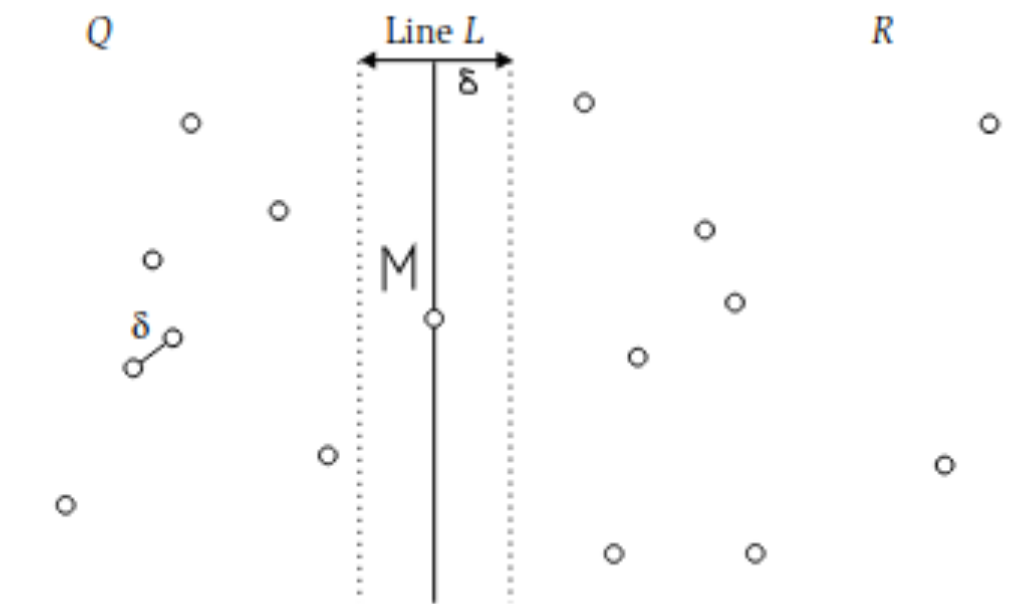
\includegraphics[width=0.6\textwidth]{points.png}
		\caption{Points in a $2D$ plane}
		\label{fig:points-png}
	\end{figure}
	We then find the minimum $L$ to $L$ distance, and similarly, we find the minimum $R$ to $R$ point distance. We also find minimum $L$ to $R$ distance. Call all these distances $d_1,d_2,d_3$. Then, the minimum distance is $min(d_1,d_2,d_3)$. However, note that, once we find $d_1$ and $d_2$, it is sufficient that we only check $\delta \eqdef min(d_1,d_2)$ to the left and right from the line $L$, since any larger numbers would mean it is larger than what we have already found. \\
	Fact. For $p_1 \in L$ and $p_2 \in R$, if $\left( p_1 \in M \lor p_2 \in M \right) $, then $d(p_1,p_2) \ge \delta$
	\begin{cor}
		It suffices to check all points $p_1 \in L$ and $p_2 \in R$ if $p_1 \in M, p_2 \in M$ then $d(p_1,p_2) < \delta$
	\end{cor}
	Fact. Remainder points of $M = \{p_1,p_2,\ldots,p_k\}$ and $y_1\le y_2\le \ldots\le y_k$
	\section{General recurrence for Divide and Conquer algorithms that are balanced}
	\begin{lstlisting}[language = pseudocode , caption={Algorithm Template} , frame = trBL , firstnumber = last , escapeinside={(*@}{@*)}]
	Divide input size (*@$A$@*) parts of size (*@$\frac{n}{B}$@*) where (*@$B \ge 2$@*)
	Solve the (*@$A$@*) parts of size (*@$\frac{n}{B}$@*) recursively
	Combine results in time (*@$O(n^c)$@*) for some constant (*@$c \ge 0$@*)
	\end{lstlisting}
	\begin{thm} If
	\begin{align*}
		T(n)\le 
		\begin{cases}
			O(1) & \text{if } n \le B \\
			A \cdot T\left( \frac{n}{B} \right) + O(n^{c}) &\text{if } > B
		\end{cases}
	\end{align*}	
	then
	\begin{align*}
		T(n) =
		\begin{cases}
			O(n^{c}) & \text{if } C > \log_B A \\
			O(n^{\log_B A}) & \text{if } C < \log_B A\\
			O(n^{c} \cdot \log n) & \text{if }C= \log_B A
		\end{cases}
	\end{align*}
	\begin{proof}
		Unfolding the recurrence tree. We draw a tree
		\begin{figure}[H]
			\centering
			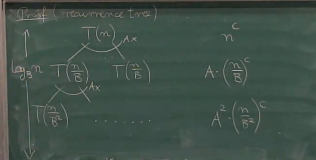
\includegraphics[width=0.6\textwidth]{tree.png}
			\caption{Recurrence Tree}
			\label{fig:tree-png}
		\end{figure}
		We have $A_i\left( \frac{n}{B_i} \right) ^{c}$ at level $i$, which can be simplified to $\left( \frac{A}{B^{C}} \right) ^{i}\cdot n^{c}$ Then,
		\begin{align*}
			T(n) = O(n^{c} \cdot \sum_{i=0}^{\log_B n} \left( \frac{A}{B^{c}} \right) ^{i}
		\end{align*}
		If $A = B^{c}$ we have $\log_B A = \log_B(B^{c)} = c$. Then,
		\begin{align*}
			\sum_{i=0}^{\log_B n} \left( \frac{A}{B^{c}} \right) ^{i} = \sum_{i=0}^{\log_B n} 1 = O(\log_B n)		\end{align*}
			Therefore we have
			\begin{align*}
				T(n) = O(n^{c} \log n)
			\end{align*}
			If we have $A < B^{c} (\log_B A < c)$, then
			\begin{align*}
				\sum_{i=0}^{\log_B A} = O(1)
			\end{align*}
			from the fact that it is a geometric series.
			It follows that then $T(n) = O(n^{c})$.\\
			If $A>B^{c} (\log_B A > c)$, then
			\begin{align*}
				\sum_{i=0}^{\log_B n} \frac{\left( \frac{A}{B^{c}} \right)^{\log_B n}-1}{\frac{A}{B^{c}}-1}
			\end{align*}
			The denominator is a constant, therefore we obtain
			\begin{align*}
				&O(\frac{A}{B^{c}\cdot\left( \frac{A}{B^{c}} \right) ^{\log_B n}}\\
				=&O(\frac{B^{\log_B A \cdot \log_B n}}{B^{c \cdot \log_B n}}) \\
				=&O(\frac{n^{\log_B A}}{n^{c}}) \\
				=&O(n^{\log_B A})
			\end{align*}
			Which implies $T(n) = O(n^{\log_B A})$
	\end{proof}
	\end{thm}
	\section{Integer Multiplication}
		Integer multiplication in computer science what may seem to be a simple problem, is actually not so simple. We will assume the multiplication is done in base $2$, although the end result does not change. We begin writing $x$ as
		\begin{align*}
			x=x_1\cdot_2^{\frac{n}{2}} + x_0
		\end{align*}
		Therefore, for the problem $xy$ we have
		\begin{align*}
			xy &= (x_1 \cdot_2^{\frac{n}{2}}+x_0)(y_1\cdot_2^{\frac{n}{2}} + y_0) \\
			   &=x_1y_1+(x_1y_0+x_0y_1)\cdot 2^{\frac{n}{2}} + x_0y_0
		\end{align*}
		This reduces the problem of solving a single $n$ bit problem instance to the problem of solving four $\frac{n}{2}$ bit instances. So we have a first candidate for a divide and conquer solution: recursively compute the results for these four $\frac{n}{2}$ bit sequences and then combine them as we have done above. Combination requires only addition, which is $O(n)$. We obtain the solution $T(n) \le O(n^{\log_2 q}= O(n^2)$. Our divide and conquer algorithm with four branching was a complicated to get back to quadratic time, if we have $q=4$. Therefore we should focus on obtaining $q=3$, i.e., try to get away with three recursive calls, resulting in $T(n) \le  O(n^{\log_2 q}) = O(n^{1.59})$. \\
		Recall that our goal is to compute the expression $x_1y_1\cdot 2^{n} + (x_1y_0+x_0y_1)\cdot 2^{\frac{n}{2}}+x_0y_0$. To make it three recursive calls, consider the result of the multiplication $(x_1+x_0)(y_1+y_0) = x_1y_1+x_1y_0+y_1x_0+x_0y_0$. This has the four products above added together, at the cost of a single recursive algorithm. If we determine $x_1y_1$ and $x_0y_0$ by recursion, we get the outermost terms explicitly, and we get the middle term by subtracting $x_1y_1$ and $x_0y_0$ away from $(x_1+x_0)(y_1+y_0)$. Therefore our algorithm is
		\begin{lstlisting}[language = pseudocode , caption={Recursive Multiply} , frame = trBL , firstnumber = last , escapeinside={(*@}{@*)}]
		(*@$x=x_1 \cdot 2^{\frac{n}{2}} + x_0$@*)
(*@$y_1 \cdot 2^{\frac{n}{2}} + y_0$@*)
		compute (*@$x_1+x_0$@*) and (*@$y_1+y_0$@*)
		(*@$p$@*) = recursiveMultiply(*@$x_1+x_0, y_1+y_0$@*)
(*@$x_1y_1 = $@*) recursiveMultiply(*@$(x_1,y_1)$@*)
(*@$x_0y_0 = $@*) recursiveMultiply(*@$(x_0,y_0)$@*)
		Return (*@$x_1y_1 \cdot 2^{n} + (p-x_1y_1-x_0y_0) + 2^{\frac{n}{2}} + x_0y_0$@*)
		\end{lstlisting}
		https://www.youtube.com/watch?v=JCbZayFr9RE
		\begin{align*}
			T(n) = \begin{cases}
				O (1) & \text{if } x,y \text{ are single digits, i.e., } n=1 \\
				3T\left( \frac{n}{2} \right) + O(n) & \text{otherwise}
			\end{cases}
		\end{align*}
		Note that $A=3$ because there are $3$ recursively calls, $c = 1$ since we combine them using only addition and subtraction, $B=2$ since we split the number into two. Therefore, we obtain asymptotic analysis of, for the case $\log_2 3 > 1$:
		\begin{align*}
			O(n^{\log_2 3})
		\end{align*}
		\section{Subset Sum and Knapsack}
		\begin{lstlisting}[language = pseudocode , caption={Subset Sum} , frame = trBL , firstnumber = last , escapeinside={(*@}{@*)}]
		Inputs: Positive integers (*@$w_1,w_2,\ldots,w_n$@*), and (*@$W$@*)
		Output: Subset (*@$S \subset \{1,2,\ldots,n\}$@*) s.t. max(*@$\left(\sum_{i \in S}^{} w_i\right)$@*) with constraint (*@$\sum_{i \in S}^{} w_i < W$@*)
		\end{lstlisting}
		Note that no correct and efficient greedy algorithms are known for such problems. We will solve this using dynamic programming and breaking it down into sub problems.
		\subsection{Sub problems}
		We can consider items from $1$ to $j$ where $j = 0,1,\ldots,n$. We can come up with a suitable recurrence.
		\begin{defn}
			\begin{align*}
			M(j) \eqdef \text{max}\left( \sum_{i \in S}^{} w_i \text{ s.t. } S \subseteq \{1,2,\ldots,j\} \land \sum_{i\in S}^{} w_i \le W \right)
			\end{align*}
		\end{defn}
		Fact. If $j$ is not in an optimal solution $S$, then $M(j) = M(j-1)$ \\
		Fact. If $j$ is an optimal solution $S$, then $M(j) = w_j + M(j-1)$ However, note that this fact is not true, as we do not consider the change in $W$, the weight. Therefore, this is subproblem does not work. Let us consider another one instead. \\
		Instead, let us consider pairs that is $\left( \{1,2,\ldots,j\}, C \right)$ where $j=0,1,\ldots,n$ and $C=0,1,\ldots,W-1,W$. We can now adjust our facts.
		\begin{defn}
			\begin{align*}
				M(j,C) \eqdef  \text{max}\left( \sum_{i \in S}^{} w_i \text{ s.t. } S \subseteq \{1,2,\ldots,j\} \land \sum_{i\in S}^{} w_i \le C \right)
			\end{align*}
		\end{defn}
		We can now rewrite our last fact.\\
		Fact. If $j$ is in an optimal solution $S$, then $M(j,C) = w_j + M(j-1,C-w_j)$ \\
		Fact.  $M(j,C)$ satisfies the following recurrence
		\begin{align*}
			M(j,C) = \begin{cases}
				0 & \text{ if } j=0 \land C = 0 \\
				M(j-1,C) &\text{if } w_j > C \\
				\text{max}\left( M\left( j-1,c \right) , w_j + M(j-1,c-w_j) \right)   & \text{if } w_j \le C
			\end{cases}
		\end{align*}
		\subsection{Compute}
		\begin{lstlisting}[language = psuedocode , caption={Computing our algorithm} , frame = trBL , firstnumber = last , escapeinside={(*@}{@*)}]
		for (*@$j=0,1,2,\ldots,n$@*) do
			for (*@$C = 0,1,2,\ldots,W$@*) do
				compute the recurrence described above
		\end{lstlisting}
		If $W$ is represented in binary/decimal, we have size of representation of $W $ as $\log_2 W$. However, $W$ is $\Omega\left( 2^{\text{size of representation of }W} \right) $. We have runtime $O(n\cdot W)$
		\section{Sequence Alignment}
		One way is to group up, for examples, a sequence such as letters. For example,
		\begin{table}[H]
			\centering
			\caption{Sequence Alignment}
			\label{tab:label}
			\begin{tabular}{|c|c|c|c|c|c|c|c|c|c|}
				\hline
				O & C & U & R & R & A &N & C & E & -  \\
				\hline
				O & C & C & U & R & R & E & N &C & E\\
			\hline

			\end{tabular}
		\end{table}
		However, with this table we have many letter mismatches. If we modify it as such:
		\begin{table}[H]
			\centering
			\caption{Sequence Alignment Redesign}
			\label{tab:sequenceredesign}
			\begin{tabular}{|c|c|c|c|c|c|c|c|c|c|}
				\hline
				O & C & - & U & R & R & A & N & C & E  \\
				\hline
				O & C & C & U & R & R & E & N &C & E\\
			\hline

			\end{tabular}
		\end{table}
		\begin{defn}
			Levenshtein, 1966. 
			\begin{align*}
				\Delta(x,y) \eqdef \text{min Cost}(A)
			\end{align*}
			where $x,y$ are letters and $A$ are different alignments of $x$ and $y$.
		\end{defn}
		\begin{defn}
			Cost. Cost of an alignment is defined to be the sum of all gap and mismatch penalties. 
		\end{defn}
		Consider $\delta$ which is gap penalty, and further, consider $\alpha_{ab\in \Sigma}$. Let $x,y \in \Sigma^{*}$ \\
		Now, let $\delta = 2$ and
		\begin{align*}
			\alpha_{ab} = \begin{cases}
			0	& \text{if } a=b\\
			1	&\text{if both $a$ and $b$ are both vowels or consonants }\\
			3	& \text{otherwise}
			\end{cases}
		\end{align*}
		\begin{lstlisting}[language = pseudocode , caption={Algorithm} , frame = trBL , firstnumber = last , escapeinside={(*@}{@*)}]
		Input: (*@$\delta, \alpha_{ab}$@*) penalties. Two words (*@$x, y$@*) with (*@$x_1,\ldots,x_m,y_1,\ldots,y_n \in \Sigma^*$@*) words respectively
		Output: (*@$ \Delta(x,y)$@*), an alignment of (*@$A \in \text{Alignments}(x,y)$@*) of min (*@$ \Delta(x,y)$@*)
		\end{lstlisting}
		\subsection{Subproblems}
		Fact. In an optimal alignment of $x$ and $y$, one of the following three cases holds:
		\begin{enumerate}
			\item Last letters of $x$ and $y$ are matched
			\item Last letter of $x$ is aligned with a gap
			\item Last letter of $y$ is aligned with a gap
		\end{enumerate}
		\begin{defn}
			The subproblems and their best solution values. For all $i=0,1,\ldots,m$ and for all $j=0,1,\ldots,n$ we define
			\begin{align*}
				D(i,j) \eqdef \Delta([x_1,x_2,\ldots,x_i],[y_1,y_2,\ldots,y_j])
			\end{align*}
		\end{defn}
		Fact. Recurrence. $D(i,j)$ satisfies the following recurrence:
		\begin{align*}
			D(i,j) = \begin{cases}
				j \cdot \delta& \text{if }i=0 \\
				i \cdot \delta & \text{if }j=0 \\
				\text{min}\{\alpha_{x_i,y_j}+D(i-1,j-1) &\text{if }i \ge 1 \land j\ge 1 \\
				\delta + D(i-1,j) & \text{if $x_i$ is aligned with a gap} \\
				\delta + D(i,j-1)\} & \text{ if $y_j$ is aligned with a gap}
			\end{cases}
	\end{align*}
	It follows that the complexity of the implementation is $O(mn)$. The space complexity is $O(m)$. However, to use linear space, we need to make observations: \\
	Fact. The solution to finding linear space is to realise that it is equivalent to understanding the bottom diagram shortest path problem.
	\begin{figure}[H]
		\centering
		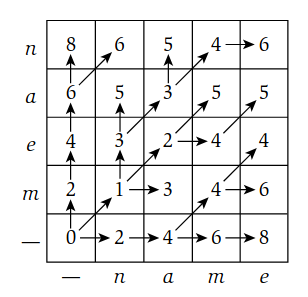
\includegraphics[width=0.35\textwidth]{diagram.png}
		\caption{NAME array}
		\label{fig:diagram-png}
	\end{figure}
	Notice that if we use horizontal edges or vertical edges it means that we use a gap. So all horizontal and vertical edges have cost $2$. $\alpha_{ab}$ denotes the weight of the edge that are slanted, depending on the letters. \\
	Fact. A min-cost alignment is a shortest path from $(0,0)$ to $(m,n)$ in the graph above.Therefore, it makes sense to find the shortest path to each vertex, and then work backwards. By doing so, we find that the best alignment is
	\begin{table}[H]
		\centering
		\caption{MEAN-NAME alignment}
		\label{tab:meanname}
		\begin{tabular}{|c|c|c|c|c|}
			\hline
		M & E & A & N & -  \\
		\hline
		N & - & A & M & E \\
		\hline
		\end{tabular}
	\end{table}
	Now notice that the maximum amount of edges we need to store is $O(m+n)$. 
	\begin{defn}
		\begin{align*}
			D(i,j) &\eqdef \Delta([x_1,x_2,\ldots,x_i],[y_1,y_2,\ldots,y_j]) \\
			E(i,j) &\eqdef \Delta([x_{i+1},x_{i+2},\ldots,x_{m}],[y_{j+1},y_{j+2},\ldots,y_{n}])
		\end{align*}
	\end{defn}
	Fact. $D(i,j)$ is the cost of the shortest path from $(0,0)$ to $(i,j)$ and $E(i,j)$ is the length of the shortest path from $(i,j)$ to $(m,n)$.\\
	Fact. The length of a shortest $(0,0)$ to $(m,n)$ path that passes through some $(\overline{i},\overline{j})$ is $D(\overline{i},\overline{j}) + E(\overline{i},\overline{j})$. \\
	If we fix some $\overline{j}$ that is arbitrary. For $\overline{j} \in \{0,1,\ldots,n\}$, if $\overline{i} \in \{0,1,\ldots,m\}$ minimizes the sum in the above fact, we have found the method to do a recurrence.
	\begin{lstlisting}[language = pseudocode , caption={Divide and conquer alignment algorithm} , frame = trBL , firstnumber = last , escapeinside={(*@}{@*)}]
	Input: two strings (*@$x,y$@*)
	If (*@$x_n =2 \lor y_m = 2$@*)
	then return algorithm naive alignment of (*@$x$@*) and (*@$y$@*)
	else compute (*@$D([x_1,x_2,\ldots,x_n],[y_1,y_2,\ldots,y_{\frac{m}{2}}])$@*)
		compute (*@$E([x_1,x_2,\ldots,x_n],[y_{\frac{m}{2}+1},\ldots,m])$@*)
		find (*@$i$@*) that minimizes (*@$D(i,\frac{n}{2})+E(i,\frac{n}{2})$@*)
		add (*@$ (i,\frac{n}{2}) $@*) to (*@$P$@*) (path)
		call divide-and-conquer alignment to (*@$i$@*)th prefix of (*@$x$@*) and (*@$\frac{n}{2}$@*) prefix of (*@$y$@*)
		call divide-and-conquer alignment to (*@$m$@*) from (*@$i+1$@*)th prefix (*@$x$@*) and (*@$n$@*) from (*@$\frac{n}{2}+1$@*)th prefix of (*@$y$@*)
	\end{lstlisting}
	\subsection{Runtime Recurrence}
	Consider $T(n,m)\le T(m-q,\frac{n}{2})+T(q,\frac{n}{2})+O(nm)$, we get the following tree:
	\begin{figure}[H]
		\centering
		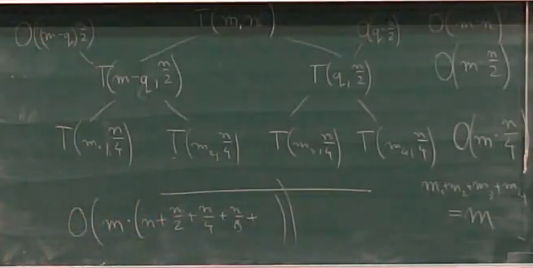
\includegraphics[width=0.8\textwidth]{trees.png}
		\caption{Tree Recurrence}
		\label{fig:trees-png}
	\end{figure}
	Notice that we get consistently $m$ but a geometric series $n$ if we sum all levels, that is,
	 \begin{align*}
		 &O(m\cdot(n+\frac{n}{2}+\frac{n}{4}+\ldots))\\
		=&O(m\cdot n \cdot \sum_{i=0}^{\infty} \frac{1}{2^{i}})\\
		=&O(2mn)\\
		=&O(mn)
	\end{align*}
	\section{Revisit to Shortest Paths}
	\begin{lstlisting}[language = pseudocode , caption={Single-Target-Shortest-Paths} , frame = trBL , firstnumber = last , escapeinside={(*@}{@*)}]
	Inputs: Directed graph with edges costs (*@$G=(V,E | c : E \mapsto \mathbb{Z})$@*) and target vertex  (*@$t \in V$@*)
	Output: If (*@$G$@*) has no negative cycles, then output for every (*@$v \in V$@*),
		output the min cost of (*@$v-t$@*) path
		output the path itself
	\end{lstlisting}
	\begin{lstlisting}[language = pseudocode , caption={Negative Cycle} , frame = trBL , firstnumber = last , escapeinside={(*@}{@*)}]
	Input: Graph with edge costs (*@$G=(V,E,c: E \mapsto \mathbb{Z})$@*) 
	Output: Yes if (*@$G$@*) has a negative cost cycle, no otherwise 
	\end{lstlisting}
	Fact. From week 3, Dijsktra fails.\\
	Fact. If $G$ has no negative cycles, then there is  min-cost $v-t$ path that is simple.
	\begin{proof}
		Let path $P$ be a min cost $v-t$ path with a cycle. Let us call the path $v-w$ the path $p'$ and $w-t$ the path $p''$. Assume a cycle $c$ exists in $w$. Notice that we can take the path $p'$ and $p''$ is also a $v-t$ path. If we do not have negative edges, then
		\begin{align*}
			c(p'+p'') = c(p') + c(p'') \le c+(p')+c(c)+c(p'')
		\end{align*}
	\end{proof}
	\subsection{Subproblems}
	\begin{align*}
		D(i,v) \eqdef min\left( c(P) : v-t \text{ path } \land P \text{ has } \le i \text{ edges } \right) 
	\end{align*}	
	Note that $i \in \{0,1,\ldots,n-1\}$ and $v \in V$. \\
	Fact. If $P$ is a mincost $v-t$ path with at most $i$ edges and $i>0$, then if $P$ has less than $i-1$ edges, then $c(P) = D(i-1,v)$. If $P$ has exactly $i$ edges and $(v,w) \in E$ and is the first edge in $D$, then the cost of the shortest path that uses at most $i$ edges and goes from $v-t$ is equal to the cost of that first edge and the optimal path from $c(v,w)+D(i-1,v)$ \\
	Fact. The following recurrence holds:
	\begin{align*}
		D(i,v) = \begin{cases}
		0	& \text{if }i=0, v=t \\
		+\infty	&\text{if }i=0, v\neq t\\
		\min(D[i-1,v], \min_{(v,w) \in E}(c(w) + D(i-1,w)))	&\text{if }i>0 \\
		\end{cases}
	\end{align*}
	\subsection{Compute}
	\begin{lstlisting}[language = psuedocode , caption={Shortest Path$(G,t)$} , frame = trBL , firstnumber = last , escapeinside={(*@}{@*)}]
	Evaluate (*@$D(i,v)$@*) for (*@$ i=0,\ldots,n-1$@*)
	Return the array (*@$(D(n-1,v))_{v \in V}$@*)
	\end{lstlisting}
	Fact. Shortest-Paths-Algorithm returns mincosts of $v-t$ paths for all $v \in V$ and runs in time $O(nm)$ and quadratic space  $O(n^2)$
	\subsection{Bellman-Ford}2
	\begin{lstlisting}[language = pseudocode , caption={The Algorithm} , frame = trBL , firstnumber = last , escapeinside={(*@}{@*)}]
	Initialise (*@$BF(v)$@*) that is (*@$0$@*) if (*@$v=t$@*), (*@$+\infty$@*) otherwise
	for (*@$i=0,1,\ldots,n-1$@*)
		for (*@$v \in V$@*) do
			BF(v) (*@$\leftarrow$@*) (*@$min(BF(v),min_{(v,w) \in E}(c(v,w)+BF(w))$@*)
	Return BF(v) for all vertices v
	\end{lstlisting}
	Fact. Correctness and complexity. At all times, $BF(v)= c(P)$ for some $v-t$ path.\\
	Fact. After iteration $i$, the value of $BF(v) \le D(i,v)$
	\subsection{Finding Mincost Paths}
	Value $BF(u)$ updated to $(c(u,w) + BF(w))$ for some $(v,w)\in E$. Let  $first(v) \leftarrow w$. \\
	Fact. If $G$ has no negative cycles, then when the Bellman-Ford algorithm terminates, got all $v \in V$, the path  $V_0$, $(v,first[V_0])$, which we call $V_1$, then $(first[V_0],first[V_1]$ and so on, we eventually arrive at $t$.\\
	Fact. Every cycle in the pointer graph is negative.
	\begin{proof}
		Along edges $(v,first[v])$ we have $BF(v) \ge c(v,w) + BF(w)$. Now consider $(v,w)$, which is the last edge to a cycle $C$ of the form $v_1,v_2,\ldots,v_k$ in the pointer graph. Just before that, we must have had that this inequality is strict, i.e., $>$ instead of $\ge $ 
		\begin{align*}
			\sum_{v \in C}^{} BF(v) &> \sum_{v \in C}^{} c(v,first(v))+BF(first(v)) \\
			0 &> c(C)
		\end{align*}
	\end{proof}
\section{From negative cycles to sink}
\begin{lstlisting}[language = psuedocode , caption={Algorithm} , frame = trBL , firstnumber = last , escapeinside={(*@}{@*)}]
Input: directed graphs (*@$G(V,E, c : E \mapsto \mathbb{Z})$@*) and (*@$t \in V$@*)
Output: A negative cycle with a path to (*@$t$@*)
\end{lstlisting}	
Fact. The following "algorithm" solves this problem 
\begin{lstlisting}[language = psuedocode , caption={A} , frame = trBL , firstnumber = last , escapeinside={(*@}{@*)}]
Input (*@$G=(V,E, c: E \mapsto \mathbb{Z})$@*)
Construct (*@$G'$@*) from (*@$G$@*) by adding (*@$t$@*) to (*@$ V'$@*) and for all (*@$ v \in V$@*) add an edge (*@$ (v,t) $@*) of cost (*@$ 0 $@*)
Return from next cycle to sink
\end{lstlisting}
Fact. $G$ has no negative cycle with a path to $t$ if and only if for all $v \in V$, $D(n-1,v) = D(n,v)$ 
\section{Intractability}
We must classify all algorithmic problems. 
\begin{align*}
	\text{TRACTABLE} \eqdef \text{Polynomial Time Solvable}
\end{align*}
The negation of the above statement is Intractable. We say that Tractable are $P$. However, there are algorithms for which we cannot prove tractable or intractable, we call these the gray zone algorithms. Some examples are Knapsack and Subset Sum. The gray area has a huge amount of classifications, however, for this module we focus only on $NP-complete$. \\
Lots of natural and important algorithmic problems have been classified as "equally hard/easy/complex", defined as $NP-complete$. To classify these problems, we use the tool called \textbf{Polynomial-time Reduction}. Polynomial time reduction allows us to compare relative complexity of algorithmic problems and has 2 key uses:
\begin{enumerate}
	\item Algorithm Design
	\item Proving Hardness
\end{enumerate}
\section{Polynomial-Time Reduction}
\begin{defn}
	If $X$ is an algorithmic problem, then an instance of $X$ is simply a legal input to $X$.
\end{defn}
\begin{defn}
	Algorithms with oracles. For $Y$ an AP, a $Y$-oracle Call is a "basic operation" that can
	\begin{enumerate}
		\item read an instance $y$ of $Y$ from a designated space in memory
		\item outputs a correct output $Y(y)$ in a designated space in memory
		\item It works in time linear in $|y| + |Y(y)|$
	\end{enumerate}
\end{defn}
\begin{defn}
	Let $X$ and $Y$ be algorithmic problems. A polynomial-time reduction from $X$ to $Y$ is a polynomial-time algorithm for $X$ that can make $Y$-oracle calls.
\end{defn}
We write $X \le_p Y$ if there exists a poly-time reduction from $X$ to $Y$.
\begin{exmp}
	A linear-time reduction from MULTIPLY to SQUARE
	\begin{lstlisting}[language = pseudocode , caption={MiltiplyBySquaring} , frame = trBL , firstnumber = last , escapeinside={(*@}{@*)}]
 (*@$AB \leftarrow SQUARE(a+b)$@*) 
 (*@$ab \leftarrow SQUARE(a-b)$@*)
 output (*@$\frac{AB-ab}{4}$@*)
	\end{lstlisting}
\end{exmp}
	Fact. Algorithm Design using reductions. Suppose $X \le_p Y$. If $Y \in P$, then $x \in P$.
	\begin{proof}
		Let $A$ be a poly-time reduction from $X$ to $Y$. Let $B$ be a poly-time algorithm for solving instances of $Y$. Let algo $A$ where all $Y \leftarrow B$ be obtained from $A$ by replacing $Y$-oracle calls by copies of $B$. The Runtime $T_{A(Y \leftarrow B)}(n) \le T_A(n) \cdot T_B(T_A(n))$. That is, from the fact that the maximum input we can put into algo $B$ is the runtime of $A$.
	\end{proof}
	We can also restate fact 5 by its negation. That is, if $X \not\in P$, then $Y \not\in P$. This means that the same fact shows us that 
	\begin{align*}
		\underbrace{X}_{\text{no harder than $Y$ }} \le_p \underbrace{Y}_{\text{no easier computationally than $X$}}
	\end{align*}
	\section{Independent Set}
	\begin{lstlisting}[language = psuedocode , caption={Algorithm} , frame = trBL , firstnumber = last , escapeinside={(*@}{@*)}]
	Inputs: Undirected graph (*@$G=(V,E)$@*), number (*@$k$@*)
	Output: Yes if (*@$G$@*) has an independent set of size (*@$k$@*), no otherwise
	\end{lstlisting}	
	\begin{defn}
		$S \subseteq V$ is independent if for all $v,w \in S$, we have $(v,w) \not\in E$, i.e., they're not connected by edges
	\end{defn}
	\section{Vertex Cover}
	\begin{lstlisting}[language = psuedocode , caption={Algorithm} , frame = trBL , firstnumber = last , escapeinside={(*@}{@*)}]
	Inputs: Undirected graph (*@$G=(V,E)$@*), number (*@$k$@*)
	Output: Yes if (*@$G$@*) has a vertex cover of size (*@$k$@*), no otherwise
	\end{lstlisting}	
	\begin{defn}
		$S \subseteq V$ is a vertex cover in $G$ if the following condition holds. For all edges $(v,w) \in E$, $v \in S$ or $w \in S$. Vertices cover edges.
	\end{defn}
	Question: Is $\text{Independent Set} \le_p \text{Vertex Covering}$ and $\text{Vertex Covering}\le_p \text{Independent Set}$. To answer, observe that
	\begin{align*}
		IS \le_p \text{MaxSize of }IS
	\end{align*}
	where $IS$ is independent set. Furthermore,
	\begin{align*}
		IS \ge_p \text{MaxSize of }IS \\
		IS \ge_p \text{A MaxSize of }IS
	\end{align*}
	Fact. In a graph $G$, $S$ is an $IS$ iff $V-S$ is a vertex cover
	\begin{proof}
		If $v \in S$ and $w \in S$, then $(w,v) \not\in S$. The negation is if $(w,v) \in S$, then $v \not\in S$ or $w \not\in S$. This is equivalent to saying if $(w,v) \in E$, then $w \in V-S$ or $v \in V-S$.
	\end{proof}
	Fact.
	\begin{align*}
		IS \le_p VC \\
		VC \le_p IS
	\end{align*}
	\begin{proof}
		We have the following poly-time reduction from $IS$ to $VC$ with algorithm $A$ of input graph $G$ and a number $k$.
		\begin{align*}
			A(G,k) = VC(G,n-k)
		\end{align*}
	\end{proof}
	\section{Set Cover}
	Input: Set $U$ of $n$ elements, a collection of subsets $s_1,s_2,\ldots,s_m$ and a positive integer k\\
	Output: If there is a collection of $k$ number of sets, such that the union of all chosen subsets are equal to $U$. \\
	Fact:
	\begin{align*}
		VC \le_p SC
	\end{align*}
	\begin{defn}
		For graph $G = (V,E)$ and $u \in V$, define $I_u = \{e \in E : u \in e\}$
	\end{defn}
	Fact. $C \subset V$ is a vertex cover in $G$ if and only if $C$ is a set cover in $E, T$ 
	\begin{proof}
	$C$ is a set cover in $E;T_n$ where $T_n$ is a family of subsets if and only if for all edges $e=(v,w)\in E$ there is some $u\in C$ such that $e \in I_u$. This simply means $v \in C$ or $w \in C$. It means that $C$ is a vertex covering, as it covers $v$ or $w$.
	\end{proof}
	Proof of the fact the poly-time reduction:
	\begin{align*}
		A((V,E),k) = SC(E,V,k)
	\end{align*}
	By fact above, SC is a yes instance of VC if and only if for all vertices $I_u$ is a yes instance.
	\section{SAT}
	Input: Boolean expressions $\phi$ in conjunctive normal form over a set of variables $X=(x_1,x_2,\ldots,x_n)$\\
	Output: Yes if and only if there is a truth assignment $V : X \mapsto \{0,1\}$ that makes expression $\phi$ true i.e., $\phi$ is satisfiable. 
	\begin{defn}
		Literal is a variable $x_i$ or its negation.
	\end{defn}
	\begin{defn}
		Clause is a disjunction of literals, e.g., $l_1 \lor l_2 \lor \ldots \lor l_k$
	\end{defn}
	\begin{defn}
		Disjunction Normal Form is a disjunction of conjunctive clauses
	\end{defn}
	\subsection{3-SAT}
	3-SAT is similar to SAT, but we restrict our inputs that in each clause we have at most $3$ literals.
	\begin{thm}
		There is a polynomial time reduction from 3-SAT to Independent Set i.e.,
		\begin{align*}
			3-SAT \le_p IS
		\end{align*}
		We pick one of the three literals occurrence in that clause and set it to $1$. While we do this we need to ensure that we avoid conflicts (i.e., we do not pick both literals $x$ and $\neg x$ in different clauses)
	\end{thm}
	\begin{exmp}
		Consider the expression
		\begin{align*}
			\phi = (\neg x_1 \lor x_2 \lor x_3) \land (\neg x_2 \lor x_1 \lor x_3) \land (\neg x_1 \lor x_2 \lor x_4)
		\end{align*}
		\begin{enumerate}
			\item We pick the occurrences $\neg x_1, x_3, \neg x_1$ 
			\item Note that there are no conflicts picked
		\end{enumerate}
		Therefore settings our picked occurrences to $1$ will satisfy our SAT. We will now create a graph $G_\phi$ using the following definition:
		\begin{defn}
			$G_\phi$. The vertices of a graph will correspond to all literal occurrences found in $\phi$. Edges will be defined in two types: Triangle edges and conflict edges. The former, for each clause we connect all $3$ pairs of literal occurrences in that clause. The latter connects all pairs of opposite literal occurrences. 
		\end{defn}
		\begin{figure}[H]
			\centering
			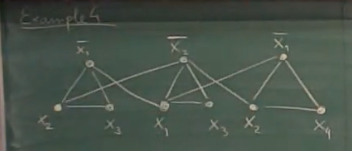
\includegraphics[width=0.8\textwidth]{one.png}
			\caption{Graph G phi}
			\label{fig:one-png}
		\end{figure}
		Note that we can not pick $2$ vertices from a single triangle. We can only pick $1$ vertex from each triangle. We need to ensure that there are no conflict edges between for the picked vertices. 
	\end{exmp}
	\begin{proof}
		Poly-time reduction from $3$-SAT to Independent set. Consider $A(\phi)$ output $I-S(G_\phi,k)$ where $\phi$ is of $k$ clauses. It is poly-time because it is routine to construct $G_\phi$ in poly time. \\
		Correctness: $\phi$ is satisfiable if and only if $G_\phi$ has an independent set of size $ k$. \\
		Suppose $X \to \{0,1\}$ satisfies $\phi$. Each clause $i$ has an occurrence of some literal $l_i$ such that $v(l_i) = 1$. For each clause $i$, let $w_i$ be the vertex in $G_\phi$ that corresponds to the literal occurrence in clause $i$. The set $\{w_1,w_2,\ldots,w_k\}$ is an independent set in $G_\phi$ because for all $i \neq j$, $v(l_i) = v(l_j) = 1$ therefore $l_i$ and $l_j$ are not opposite literals so $\{w_i,w_j\}$ is not a conflict edge. \\
		For the second implication, let $\{w_1,w_2,\ldots,w_k\}$ be an independent set in $G_\phi$ where $w_i$ is from $i$-th triangle. The corresponding literal occurrences are in distinct clauses. Let $l_i$ be the literal in the $i$-th clause. We define truth assignment $v:X \to \{1,0\}$ by setting $v(l_1)=v(l_2)=v(l_3) = 1$. $v$ is well defined, because for all $i \neq j$ therefore $\{w_i,w_j\}$ is not a conflcit edge $l_i$ and $l_j$ are not opposites. $\phi$ is satisfied by $v$, because every clause literal is $1$.
	\end{proof}
	\section{Certification and NP}
	\begin{defn}
		If $X$ is an algorithmic decision problem (ADP), let $x$ be an instance of $X$. We write $x \in X$ as shorthand for the statement that $x$ is a YES instance of $X$. Let $A(x)$ be a poly-time algorithm for an algorithmic decision problem $X$ if there is a polynomial $q(n)$ such that its running time is bounded by $q(|x|)$ where $|x|$ is number of bits. $x \in X$ iff $A(x) =$ YES. 
	\end{defn}
	\begin{align*}
		P \eqdef \{ X \in ADP : \text{ there is a poly-time algorithm} \}
	\end{align*}
	All the problems we covered thus far, there was no poly-time algorithm discovered to solve them efficiently. No one knows how to prove that no poly-time algorithm exists. For all YES instances, there is a short (POLY-SIZED) solution that can be checked (certified) in polynomial time. 
	\begin{defn}
		A certifier for a ADP $X$ is a algorithm $A(x,c)$ where $x$ is an instance and $c$ is a certificate such that $x$ is a YES instance iff there exists a string $c$ such that $A(x,c) = $ YES. The poly-time version of this definition requires an additional condition: there is a polynomial $p$ such that $x$ is a YES instance there exists a string $|c| < p(|x|)$.
	\end{defn}
	\begin{exmp}
		3-SAT certifier. The certified cert-$3$-SAT$(p,v)$ where $p$ is the instance $v$ is the certificate. The output is YES if $\phi$ evaluates to  $1$ for truth asignment $v$. Output NO otherwise.  \\
		It takes poly-time to evaluate $\phi$ for $v$. \\
		Correctness. If $\phi \in 3$-SAT, then there is vars of $\phi \to (0,1)$ such that $v(\phi) = 1$. If $\phi$ is not in $3$-SAT, then for all truth assignments variables of $\phi$ we have $v(\phi) = 0$. 
	\end{exmp}
	\begin{exmp}
		Certifier of Independent Set. $Cert-I-S((G,k),S)$ where $S$ is a set of vertices. The certifier will output YES if $S$ has size $k$ and $S$ is an independent set in $G$. NO otherwise. \\
		We first need to ensure it can be CONVINCED - outputs a YES when it's a YES. \\
		The certificate CANNOT BE FOOLED into answering YES for a NO instance
	\end{exmp}
	\begin{align*}
		NP \eqdef \{ X \in ADP : \text{ there is a poly-time certifier for }X\}
	\end{align*}
	\begin{thm}
		$P \subseteq NP$
	\begin{proof}
		Let $X \in P$, meaning that $A(x)$ for solving instances of $X$ in poly-time. Then the following $A$-cert$(x,c)$: output $A(x)$ is a correct poly-time certifier for $X$.
	\end{proof}
	\end{thm}
	\begin{defn}
		A ADP $X$ is NP-Complete if
		\begin{enumerate}
			\item $X \in NP$ 
			\item $\forall Y \in NP$, we have $Y \le_p X$
		\end{enumerate}
	\end{defn}
	\begin{cor}
		For every NP-complete ADP $X$ :
		\begin{align*}
			X \in P \iff P = NP
		\end{align*}
	\end{cor}
	\begin{thm}
		CircuitSAT is NP-Complete. In CircuitSAT the inputs are Boolean Circuits. The output is YES iff there is a truth assignment to none-fixed circuit input such that the circuit evaluates to $1$. 
	\end{thm}
	Fact. Suppose $Z$ is NP-Complete, then any problem $X$ is NP-Complete if $X \in NP$ and $Z \le_p X$
	\begin{thm}
		$3$-SAT is NP-Complete.
		\begin{proof}
			We have designed a certifier for $3$-SAT therefore we know it is NP-easy. To show that it is NP-hard, we consider
			\begin{align*}
				CircuitSAT \le_p 3-SAT
			\end{align*}
			We construct a CNF $\phi$ such that the circuit $k$ is satisfiable if and only if our CNF $\phi$ is satisfiable. 
		\end{proof}
	\end{thm}
	\begin{cor}
		Independent Set, Set Cover, Vertex Cover are all NP-Complete. 
	\end{cor}
	\section{Network Flow}
	\begin{defn}
		Matching. $M \subseteq E$ is a MATCHING in graph $G=(V,E)$ if $\forall e,f \in E$ where $e \neq f$ we have $e \cap f = \varnothing$
	\end{defn}
	\begin{defn}
		A graph $G=(V,E)$ is bipartite if
		\begin{enumerate}
			\item $V = L \cup R$ such that $L \cap R = \varnothing$
			\item $\forall e \in E$ such that $e \cap R \neq \varnothing$ and $e \cap L \neq \varnothing$
		\end{enumerate}
	\end{defn}
	\begin{defn}
		Flow Network is a directed graph $G$ with two distinguished vertices $S$ (source) and $T$ (sink) and edge capacities $c : E \to \mathbb{Z}$. Flow networks model transportation networks. I.e., $S$ is where the traffic is given and $T$ is where the traffic is supposed to get to.
	\end{defn}
	\begin{defn}
		Flow is a function $f : E \to \mathbb{R}^{+}$. It must, however, abide the capacity constraint. I.e., $\forall  e \in E$, $0 \le f(e) \le c(e)$. Furthermore, for every $ v \in V - \{S,T\}$ it must be that $v_{in}=v_{out}$
	\end{defn}
	\begin{defn}
		\begin{align*}
			val(f) \eqdef f^{out}(S)
		\end{align*}
	\end{defn}
	\subsection{Max Flow}
	Inputs: Flow networks $G=(V,E,s,t,c)$ \\
	Output: Flow $f : E \to \mathbb{R}^{+}$ of maximum value.\\
	\begin{defn}
		Residual graph $G_f$ of flow $f$ in network $G=(V,E,s,t,c)$ is a graph of vertices $V$ and two types of edges:
		\begin{enumerate}
			\item $\forall e \in E$ s.t. $f(e) < c(e)$ we have the forward edge $e $ with residual capacity $c_f(e) = c(e) - f(e)$. 
			\item $\forall  e = (v,w) \in E$ such that $f(e) > 0$ the backwards edge  $e'=(w,v)$ has residual capacity $c_f(e') = f(e) > 0$
		\end{enumerate}
		\begin{figure}[H]
			\centering
			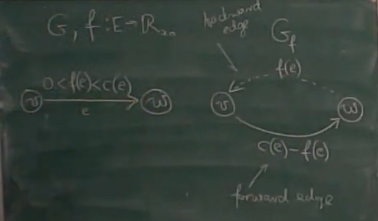
\includegraphics[width=0.6\textwidth]{two.png}
			\caption{Graph $G_f$}
			\label{fig:two-png}
		\end{figure}
	\end{defn}
	\begin{defn}
		\begin{align*}
			\text{Bottleneck}(P,f) \eqdef \text{Min residual capacity of edges in path $P$ in $G_f$}
		\end{align*}
	\end{defn}
	\begin{defn}
		\begin{align*}
			\text{Augment}(f,P)
		\end{align*}
		\begin{lstlisting}[language = pseudo , caption={Augment} , frame = trBL , firstnumber = last , escapeinside={(*@}{@*)}]
		B (*@$\leftarrow$@*) Bottleneck(P,f)
		for (*@$e \in P$@*) do 
			if (*@$e$@*) is a forward edge
				(*@$f(e) \leftarrow f(e) + B$@*)
			if (*@$e$@*) is a backward edge
				(*@$ f(\overleftarrow{e}) \leftarrow \overleftarrow{e} - B$@*)
		output((*@$f$@*))
		\end{lstlisting}
		where if $e = (v,w)$ then $\overleftarrow{e} = (w,v)$
	\end{defn}
	Fact. If $f$ is a flow in $G$ and $P$ is a $s-t$ path in $G_f$ ("an augmenting path") then $f'=Augment(f,P)$ is a flow in $G$ and $val(f') = val(f) + B$ \\
	\subsection{Ford-Fulkerson}
	Input $((V,E),s,t,c : E \to \mathbb{Z})$\\
	Initialise $f(e) = 0$ for all $e \in E$. \\
	while there is an $s-t$ path in $G_f$ do\\
	$f \leftarrow Augment(f,P)$ \\
	output($f$)		\\		
	Fact. Integrality Invariant. Throughout $F-F$ the following are integers:
	\begin{enumerate}
		\item Flow values $f(e)$ for all $e \in E$ 
		\item Residual capacities $c_f(e)$ for all $e \in E_f$
	\end{enumerate}
	\begin{thm}
		Suppose all capacities are integers. Then $F-F$ terminates after at most 
		\begin{align*}
			C \eqdef \sum_{e \in out(S)}^{} c(e)
		\end{align*}
		iterations. Therefore, $F-F$ can be implemented to be run in $O(mC)$ time.
	\end{thm}
	\subsection{Max Flows and Min Cuts}
	\begin{defn}
		$s-t$ cut. $(A,B)$ is an $s-t$ cut if $A \cup B = V \land A \cap B = \varnothing$. We also $S \in A$ and $T \in B$. The capacity of an $s-t$ cut $(A,B)$ is 
		\begin{align*}
			cap(A,B) = \sum_{e \in out(A)}^{} c(e)
		\end{align*}
	\end{defn}
	Fact. Suppose $f$ is a flow and $(A,B)$ is an $s-t$ cut. Then
	\begin{align*}
		v(f) &= f^{out}(A) - f^{in}(A) \\
		     &= \sum_{e \in out(A)}^{} f(e) - \sum_{e\in in(A)}^{} f(e)
	\end{align*}
	Note that $(\{s\}, V-\{s\})$ is still an $s-t$ cut. 
	\begin{cor}
		Weak Duality. For all flows $f$ and $s-t$ cuts $(A,B):$ 
		\begin{align*}
			v(f) \le cap(A,B)
		\end{align*}
		\begin{proof}
			$v(f) = f^{out}(A) - f^{in}(A)$ from fact two. Notice that 
\begin{align*}
	v(f) &\le f^{out}(A) \\
	     &= \sum_{e \in out(A)}^{} f(e) \\
	& \le  \sum_{e \in out(A)}^{} c(e) \\
	&= cap(A,B)
\end{align*}
		\end{proof}
	\end{cor}
		Mincut\\
		The input is a flow network $((V,E),s,t,c)$ \\
		The output is an $s-t$ cut of the min capacity. \\
		\begin{cor}
			If $val(f) = cap(A,B)$ then by weak duality $f$ is a max value flow and $(A,B)$ is a min capacity $s-t$ cut.
		\end{cor}
		Fact.
		\begin{align*}
			\text{Max Flow Value } =\text{ Min Cut Cap}
		\end{align*}
		This is called the strong duality theorem. 
		\begin{thm}
			Augmenting Path Theorem. Flow $f$ has max value if and only if its residual graph $G_f$ has no augmenting path.
			\begin{proof}
				We show that there is an $s-t$ cut $(A,B)$ such that its capacity is equal to flow $f$, $f$ is a max value flow, the residual graph has no augmenting paths are all equivalent statements. The first two statements are implied with weak duality. We show that second statement implies third statement. Proof by contrapositive. Assume there is an $s-t$ path in the residual graph called path $P$. We augment that graph to obtain flow  $f'$ we obtain hat $v(f') > v(f)$. We see that the second statement does not hold as $f$ is not a unsure. We show that third statement implies first. Suppose that there is no $s-t$ path in the residual graph. If we define $A$ to be the set of vertices such that there is a path to $v$ from $s$ in the residual graph, then $(A,B)$ is an $s-t$ cut. 
			\end{proof}`
		\end{thm}
		\begin{cor}
			$F-F$ returns outputs a max value flow. $F-F$ can also output a min-capacity $s-t$ cut with extra $O(n)$ time. 
		\end{cor}
		Fact. If all edge capacities are integers, then $F-F$ returns an INTEGRAL FLOW. 
	\subsection{Max Bipartite Matching}
	Input: Bipartite graph $G$ \\
	Output: Maximum size matching in $G$
	A matching is maximising the amount of nodes are used. To create this, we make a bipartite graph into a flow. We copy all the vertices and edges. We now add a $s$ and a $t$ vertex. The $s $ vertex connects to all $L$ and $t $ connects to all $R$. We make a direction for all vertices from left to right. The capacities are all $1$. \\
	\begin{figure}[H]
		\centering
		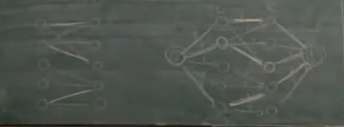
\includegraphics[width=0.5\textwidth]{three.png}
		\caption{Constructed Flow Network from Bipartite Graph}
		\label{fig:three-png}
	\end{figure}
	Fact. For every matching $m$ in $G$ there is an integral flow $f'_m$ such that $|m| = v(f'_m)$\\
	Fact. For every integral flow  $f$ in $G$, there is a matching $M_f$ in graph $G$ such that the value of $f = |M_f|$
	\begin{lstlisting}[language = pseudo , caption={FFMaxMatching} , frame = trBL , firstnumber = last , escapeinside={(*@}{@*)}]
	Construct flow network (*@$\bar{G}$@*)
	(*@$f^* \leftarrow FF(\bar{G})$@*)
	Output (*@$M_{f^*}$@*)
	\end{lstlisting}
	If $f^{*}$ is a max value flow of $\bar{G}$ then $M_{f^{*}}$ is a max size matching in $G$. However, the capacity here is bounded by the number of vertices $V$ as capacities are always $1$. Therefore, FFMaxMatching has runtime $O(nm)$
	\begin{thm}
		Define $N(A) = \{v \in V : \text{ there is $a \in A$ s.t. $(a,v) \in E$} \}$ \\
		 Fact. If there is $A \subseteq L$ such that $|N(A)| < A$ then bipartite graph $G = (L \cup R, E) $ does not have a perfect matching. The inverse is also true. This is called Hall's Marriage Problem. If you take a bipartite graph $G$ such that $|L| = |R|$ then $G$ having a perfect matching is equivalent to $\forall A \subseteq L$, we have $|N(A)| \ge |A|$
	\end{thm}
\end{document}

